\documentclass[letterpaper, 11pt]{article}
%% ================================
%% Packages =======================
\usepackage[utf8]{inputenc}      %%
\usepackage[T1]{fontenc}         %%
\usepackage{lmodern}             %%
\usepackage[spanish]{babel}      %%
\decimalpoint                    %%
\usepackage{listings}
\usepackage{fullpage}            %%
\usepackage{fancyhdr}            %%
\usepackage{graphicx}            %%
\usepackage{amsmath}             %%
\usepackage{color}               %%
\usepackage{mdframed}            %%
\usepackage[colorlinks]{hyperref}%%
\usepackage{wrapfig}             %%
\usepackage{enumitem}            %%
\usepackage{textcomp}            %%
\usepackage{gensymb}             %%
\usepackage{float}
\usepackage{xcolor}
%% ================================
%% ================================

%% ================================
%% Page size/borders config =======
\setlength{\oddsidemargin}{0in}  %%
\setlength{\evensidemargin}{0in} %%
\setlength{\marginparwidth}{0in} %%
\setlength{\marginparsep}{0in}   %%
\setlength{\voffset}{-0.5in}     %%
\setlength{\hoffset}{0in}        %%
\setlength{\topmargin}{0in}      %%
\setlength{\headheight}{54pt}    %%
\setlength{\headsep}{1em}        %%
\setlength{\textheight}{8.5in}   %%
\setlength{\footskip}{0.5in}     %%
%% ================================
%% ================================

%% =============================================================
%% Headers setup, environments, colors, etc.
%%
%% Header ------------------------------------------------------
\fancypagestyle{firstpage}
{
  \fancyhf{}
  \lhead{
\includegraphics[height=4.5em]{dcc}}
  \rhead{CC3501-1 \semestre\\
         Métodos Numéricos para la Ciencia e Ingeniería\\
         Prof.: \profesor}
  \fancyfoot[C]{\thepage}
}

\pagestyle{plain}
\fancyhf{}
\fancyfoot[C]{\thepage}
%% -------------------------------------------------------------
%% Environments -------------------------------------------------
\newmdenv[
  linecolor=gray,
  fontcolor=gray,
  linewidth=0.2em,
  topline=false,
  bottomline=false,
  rightline=false,
  skipabove=\topsep
  skipbelow=\topsep,
]{ayuda}
%% -------------------------------------------------------------
%% Colors ------------------------------------------------------
\definecolor{gray}{rgb}{0.5, 0.5, 0.5}
%% -------------------------------------------------------------
%% Aliases ------------------------------------------------------
\newcommand{\scipy}{\texttt{scipy}}
\newcommand{\newtitle}[1]{\noindent\Large{\textbf{#1}}\\\vspace*{-0.5em}\normalsize}
%% Propiedades compilación pdf
%% -------------------------------------------------------------
%% =============================================================
%% =============================================================================
%% CONFIGURACION DEL DOCUMENTO =================================================
%% Llenar con la información pertinente al curso y la tarea
%%
\newcommand{\tareanro}{1}
\newcommand{\fechaentrega}{15/04/19 23:59 hrs}
\newcommand{\semestre}{2018A}
\newcommand{\profesor}{Nancy Hitschfeld K.}
%% =============================================================================
%% =============================================================================
\hypersetup{
	bookmarksopen={false},
	pdfauthor={Nancy Hitschfeld K.},
	pdfcreator={LaTeX},
	pdfdisplaydoctitle={true},
	pdfkeywords={Computación Gráfica, CC3501-1},
	pdflang={es-CL},
	pdfmenubar={true},
	pdfremotestartview={Fit},
	pdfpagelayout={OneColumn},
	pdfpagemode={UseNone},
	pdfstartpage={1},
	pdfstartview={FitH},
	pdfsubject={Computación Gráfica},
	pdftitle={Tarea \tareanro},
	pdfview={FitH}
}
\pdfminorversion=7
\hfuzz=200pt \vfuzz=200pt
\hbadness=\maxdimen \vbadness=\maxdimen

% Definición de colores
\definecolor{backcolour}{rgb}{0.95, 0.95, 0.92}
\definecolor{codegray}{rgb}{0.5, 0.5, 0.5}
\definecolor{codegreen}{rgb}{0, 0.6, 0}
\definecolor{codepurple}{rgb}{0.58, 0, 0.82}
\definecolor{dgray}{rgb}{0.35, 0.35, 0.35}
\definecolor{dkgreen}{rgb}{0, 0.6, 0}
\definecolor{gray}{rgb}{0.5, 0.5, 0.5}
\definecolor{lbrown}{RGB}{255, 252, 249}
\definecolor{lgray}{RGB}{180, 180, 180}
\definecolor{lyellow}{rgb}{1.0, 1.0, 0.88}
\definecolor{mauve}{rgb}{0.58, 0, 0.82}
\definecolor{mygray}{rgb}{0.5, 0.5, 0.5}
\definecolor{mygreen}{rgb}{0, 0.6, 0}
\definecolor{mylilas}{RGB}{170, 55, 241}
\definecolor{ocre}{RGB}{243, 102, 25}

\lstdefinestyle{Python}{
	language=Python,
	aboveskip=3mm,
	backgroundcolor=\color{backcolour},
	basicstyle={\small\ttfamily},
	belowskip=3mm,
	breakatwhitespace=false,
	breaklines=true,
	columns=flexible,
	commentstyle=\color{codegreen},
	keepspaces=true,
	keywordstyle=\color{magenta},
	numbers=left,
	numbersep=5pt,
	numberstyle=\tiny\color{codegray},
	showspaces=false,
	showstringspaces=false,
	showtabs=false,
	stepnumber=1,
	stringstyle=\color{codepurple},
	tabsize=3
}
\renewcommand{\lstlistingname}{Código} % Nombre leyenda del código fuent

\begin{document}
\thispagestyle{firstpage}

\begin{center}
  {\uppercase{\LARGE \bf Tarea \tareanro}}\\
  Fecha de entrega: \fechaentrega
\end{center}


%% =============================================================================
%% ENUNCIADO ===================================================================
\newtitle{Problema}

En una región del litoral central Chileno se planea construir una planta
industrial destinada a la refinación del petróleo. El diseño propuesto
considera una gran emisión de calor a la atmósfera, por lo cual en la
evaluación de impacto ambiental se le pide a usted, como alumno del curso de computación gráfica, modelar el comportamiento térmico de la atmósfera con la planta en operación. \\

\begin{wrapfigure}{r}{0.6\textwidth}
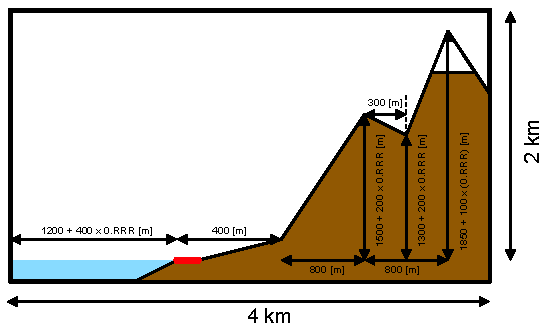
\includegraphics[width=0.6\textwidth]{perfil.pdf}
\end{wrapfigure}

\par Se le pide modelar un perfil del litoral (corte transversal en dirección
Este--Oeste) de 4 [km] de ancho y 2 [km] de alto parecido al de la figura. La
planta se ubicará en la playa (entendida como el borde entre el mar y las
montañas; en la figura se indica por una franja roja).

Por simplicidad consideraremos que la temperatura de la atmósfera cumple la
ecuación de Poisson:
$$
\frac{\partial^2 T(x, y)}{\partial x^2} +
\frac{\partial^2 T(x, y)}{\partial y^2} = \rho(x,y)
$$
\\
En donde $\rho(x,y)$ es una función cualquiera que depende de la distancia $(x,y)$ con respecto al centro de la planta. Nótese que si $\rho(x,y)=0$ se tiene la ecuación de Laplace vista en clases.

\vspace{0.5cm}
\newtitle{Condiciones de borde}

La temperatura de la superficie del mar varía a lo largo del día de acuerdo a
la siguiente receta: T = 4\textordmasculine C entre las \texttt{00:00} y las
\texttt{08:00} hrs; luego T aumenta linealmente hasta alcanzar los
20\textordmasculine C a las \texttt{16:00}; y finalmente T decrece linealmente
hasta alcanzar T=4\textordmasculine C a las \texttt{24:00} (Ver figura \ref{temp} del anexo). Para el problema asumiremos que la temperatura superficial del mar varía en la forma descrita independiente de la temperatura atmosférica.

La temperatura de la atmósfera (en ausencia de fuentes de calor que no sean la
superficie del mar) varía en el tiempo igual que la temperatura en la
superficie del mar pero además decae linealmente en 6\textordmasculine C cada
1000 [m]. Asumiremos que nuestra caja es suficientemente grande para que los
bordes de nuestro perfil no se vean afectados por la planta industrial.

Por su parte, la temperatura del suelo en la región continental es constante e
igual a 20\textordmasculine C todo el día, excepto por sobre los 1800 [m],
donde hay nieve (que consideraremos a 0 \textordmasculine C).

En cuanto a la planta, esta tiene chimeneas que cubren un ancho de 120 [m]
ubicada al nivel del mar. El comportamiento térmico de la chimenea a lo largo
del día esta descrito por la siguiente expresión (como función de la hora $t$):

$$
T = 450 \left(  \cos\left( \frac{\pi}{12}\cdot t \right) + 2 \right)
\quad [{\rm \degree C}];\ t \in [0,24]
$$

\newtitle{Geografía}

El perfil geográfico a estudiar está detallado en la figura y contiene algunos
elementos aleatorios que dependen de \texttt{RRR} (los últimos 3 dígitos de su
\texttt{RUT}, antes del dígito verificador). En particular:

\begin{itemize}[label={--}]
	\item Partiendo del Oeste, la superficie del mar cubre $1200 + 400 \times
	0.\texttt{RRR}$ [m].
	\item A partir del borde costero, la planta industrial tiene chimeneas
	cubriendo un ancho plano de 120 [m] (la región roja de la figura).
	\item Luego de la planta hay una inclinación suave que aumenta 100 [m] de
	altura por cada 300 [m] que se recorre hacia el Este. Esta inclinación llega
	hasta 400 [m] a partir del borde costero.
	\item Luego de la pequeña inclinación, viene la cordillera de la costa
	que caracterizamos por dos cimas triangulares. La primera tiene una altura
	máxima de $1500 + 200 \times 0.\texttt{RRR}$ [m], la cual se ubica a 1200 [m]
	de la orilla del mar.
	\item A continuación hay un punto de menor altura: $1300 + 200
	\times\texttt{0.RRR}$ [m], el cual se ubica a 1500 [m] de la orilla del mar.
	\item Luego viene una segunda cima, más alta que la primera que alcanza
	$1850 + 100 \times 0.\texttt{RRR}$ [m] a 2000 [m] desde la orilla del mar.
	Recuerde que todos los puntos de la superficie que están a más de 1800 [m]
	están cubiertos de nieve a 0 \textordmasculine C.
	\item Decida Ud. qué hacer con el tramo que falta.
\end{itemize}

\vspace{0.5em}
\newtitle{Requerimientos específicos}

\par \indent A continuación una lista de requerimientos mínimos para su informe:
\begin{itemize}[label={--}]
	\item Describa su estrategia de discretización del espacio.
	\item Describa qué tipo de condiciones de borde se necesitan de acuerdo a
	la descripción del problema. ¿Cómo las implementó en su solución?
	\item Determine la temperatura atmosférica para $t = 0, 8, 12, 16, 20$
	[hrs].
	\item Resuelva el problema usando el \textbf{método de la sobre-relajación
		sucesiva}. Explore el valor más óptimo para el parámetro $w$.
\end{itemize}

\vspace{0.5em}
\newtitle{Instrucciones Importantes}
\begin{itemize}
\item Al hacer el informe usted debe decidir qué es interesante y
  agregar las figuras correspondientes. No olvide anotar los ejes, las unidades e incluir una \emph{caption} o título que describa el contenido de cada figura.
  
 \item No olvide indicar su RUT en el informe.

 \item Repartición de puntaje: 50\% implementación y resolución del problema; 50\% calidad del reporte entregado: demuestra comprensión del problema y su solución, claridad del lenguaje, calidad de las figuras utilizadas.

 \item \textbf{IMPORTANTE.} En esta tarea nos importa mucho su análisis del
   problema. Del 45\% contenido en el ítem ``calidad del reporte'', 15\%
   corresponde a su introducción, descripción del problema, descripción de su
   implementación, ortografía, etc., el otro 30\% corresponden a su análisis
   del resultado: ¿Tienen sentido sus resultados?  ¿Por qué sí, o por qué no?
   ¿Cuál es el efecto del mar en el sistema? ¿A qué horas se obtiene la menor
   temperatura media del sistema? ¿Cuál podría ser una estrategia para reducir
   el impacto de la planta en el medio ambiente?

\end{itemize}

\vspace{0.5em}
\newtitle{Anexos}

\begin{figure}[H]
	\centering
	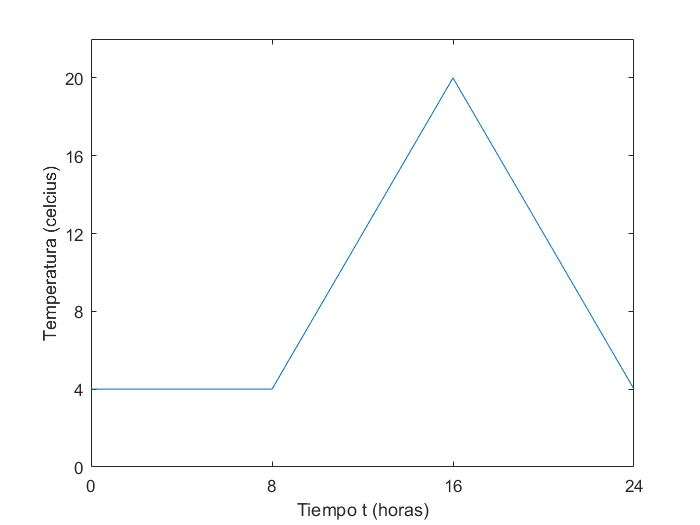
\includegraphics[width=8cm]{temperatura}
	\label{temp}
	\caption{Variación de temperatura del sistema}
\end{figure}

\lstset{
	style=Python
}
\begin{lstlisting}[language=Python,caption={Ejemplo paso función por argumento}]
def rho(x, y):
	return x * y
	
...

def iniciarIteracion(f):
	...
	matriz[i][j] = f(i/h, j/h)	# h dimension grilla
	
...

iniciarIteracion(rho)	# Se pasa la funcion rho por variable
\end{lstlisting}

%% FIN ENUNCIADO ===============================================================
%% =============================================================================

\end{document}
